%\documentclass[red, hyperref={pdfpagelabels=false}]{beamer}
\documentclass[red]{beamer}
\hypersetup{pdfpagemode=FullScreen}

\mode<presentation>
\usepackage{beamerthemesplit}
\usepackage[T1]{fontenc}
\usepackage{textcomp}
\usepackage{lmodern}
%\usepackage{listings,bera}
%\usepackage{color}

%\usetheme{boxes}
%\usetheme{Darmstadt}
\usetheme{Dresden}
%\usetheme{Frankfurt}
%\usetheme{Ilmenau}
%\usetheme{Madrid}
%\usetheme{Warsaw}

\title{Examining the Errors in Dual-Polarization Attenuation Correction}
\author{Ryan May}
%\institute{ARRC}
\date{27 February 2014}
\titlegraphic{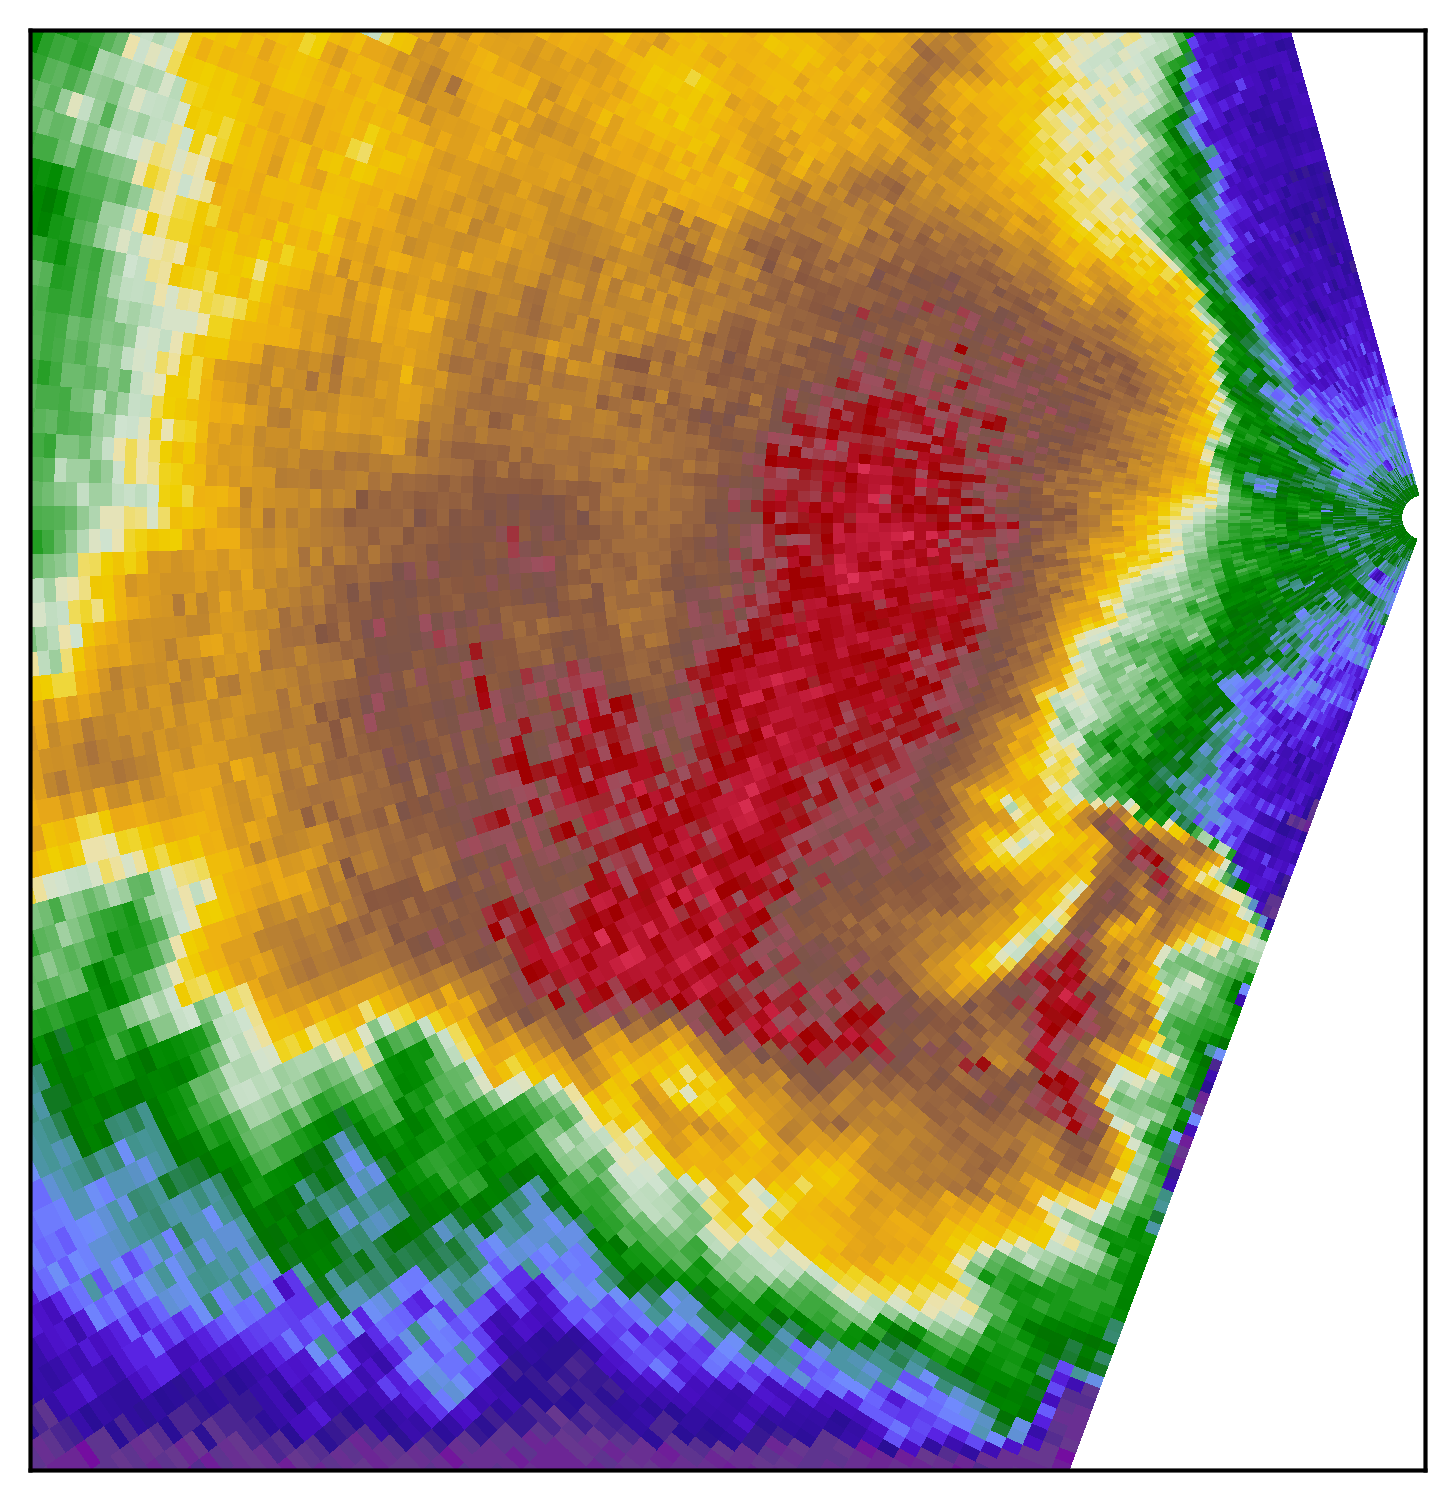
\includegraphics[scale=0.17]{figures/title_ppi.png}}

\begin{document}

\begin{frame}
\titlepage
\end{frame}
%\frame{\titlepage}

\section[Outline]{}
\begin{frame}{Outline}
    \tableofcontents
\end{frame}

\section{Motivation}
\stepcounter{subsection}
\begin{frame}
	\frametitle{Attenuating Systems}
	\begin{itemize}
		\item Proliferation of systems at attenuating wavelengths (C and X bands)
		\item Can be cheaper
		\item Better angular resolution
		\item Better sensitivity
	\end{itemize}
\end{frame}

\begin{frame}
	\frametitle{Applications}
	\begin{itemize}
		\item Any quantitative use of the data necessitates data correction
		\item QPE
		\item Hydrometeor Classification
		\item 3dB error -> 64\% change in rain rate
	\end{itemize}
\end{frame}

\section{Simulation}
\stepcounter{subsection}
\begin{frame}
  \frametitle{Simulator}
  \begin{itemize}
  	\item Model provides needed environmental information
  	\only<2>{ \begin{itemize}
  		\item Hydrometeor content
  		\item Wind components
  		\item Thermodynamic information
  		\end{itemize} }
  	\item Propagate discretized radar pulse through simulation grid
  	\item During propagation, accumulate phase shift and attenuation
  	\item Calculate scattering parameters from hydrometeor information and temperature
  	\item Use scattering together with radar equation to synthesize radar signal
  	\item Includes antenna pattern (with optional sidelobes), range weighting, and noise
  	\item Also calculate some volume integrated quantities (e.g. attenuation)
  \end{itemize}
\end{frame}

\begin{frame}
	\frametitle{Signal Synthesis}
	\begin{itemize}
		\item Each pulse element gets assigned values from the model grid using nearest
		neighbor sampling
		\item Start each element with uniformly distributed random phases
		\item Each element functions as "scattering center" that generates
		a phase shift (Muschinski 1999)
		\item Power at each element is exponentially distributed with expected value
		given from scattering 
		\item Correlation between polarizations uses scattering calculation
		to adjust randomness between polarizations (Galati 1995)
		\item Each polarization is attenuated and phase-shifted separately
		\item Altogether, this gives complex, random values for each pulse element for 
		each polarization
		\item These are summed and added to white noise for an IQ sample for the pulse
	\end{itemize}
\end{frame}

\begin{frame}
	\frametitle{Scattering}
	\begin{itemize}
		\item Configurable scattering models
		\begin{itemize}
			\item T-Matrix
			\item Rayleigh-Gans
			\item Mie
			\item Rayleigh
			\end{itemize}
		\item Configurable drop shape model
		\begin{itemize}
			\item Brandes et al. (2004) polynomial model
			\item Pruppacher and Beard (1970) linear model
			\end{itemize}
		\item Wavelength- and temperature-dependent complex dielectric constant
		\item Width of canting angle distribution can also be controlled
	\end{itemize}
\end{frame}

\begin{frame}
	\frametitle{Microphysics}
	\begin{itemize}
		\item Native model microphysics scheme is two-moment (Ziegler 1985)
		\item Model distribution is a gamma distribution for volume of drops
		\item However this distribution is not well-suited to radar
		\item Use modified gamma distribution on diameter ($\mu=1.8102$)
		\item This uses the model's number concentration and liquid water content
		\item Also conserves model's $D^6$ (or $V^2$)
	\end{itemize}
\end{frame}

\begin{frame}
	\frametitle{Microphysics (cont.)}
	\centering{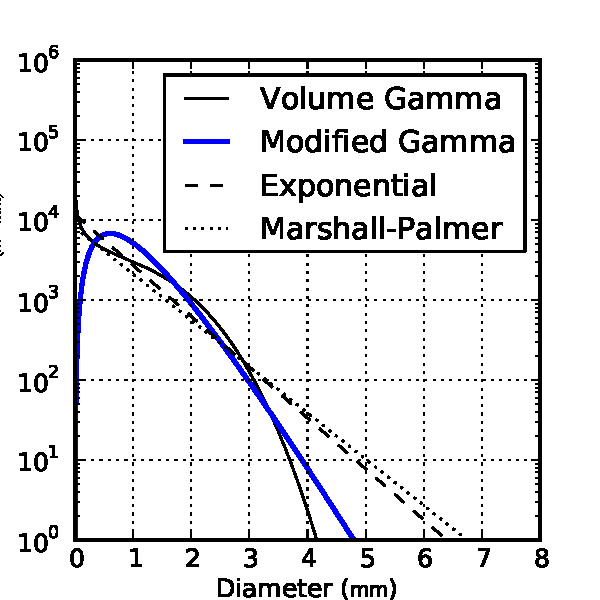
\includegraphics[scale=0.6]{figures/distribution-comparison.pdf}}
\end{frame}

\begin{frame}
	\frametitle{Model Field}
	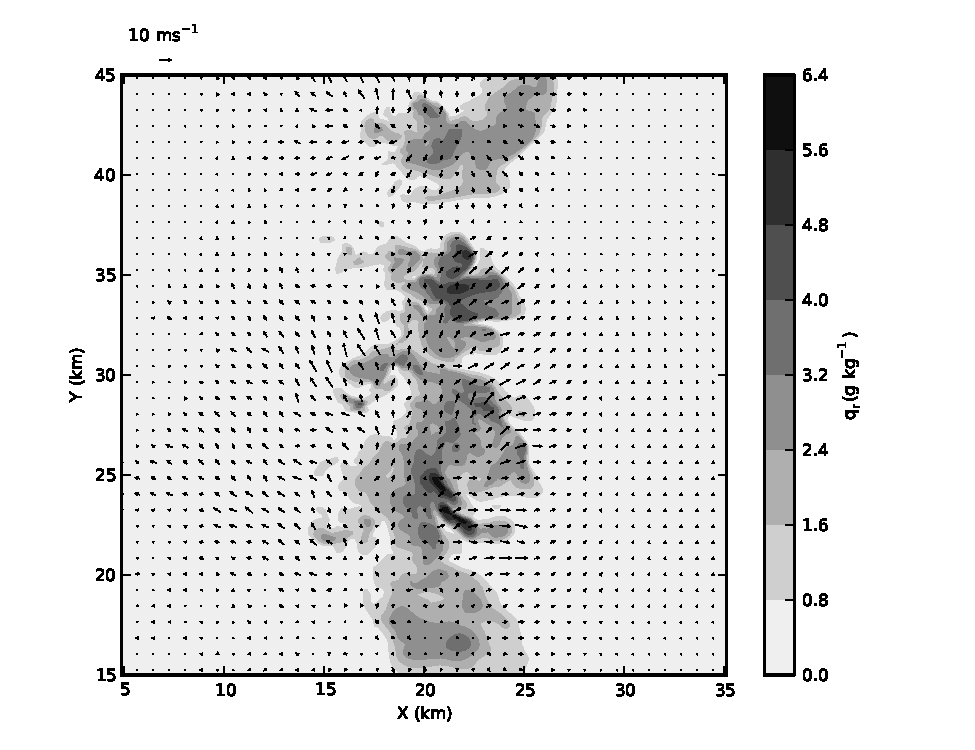
\includegraphics[scale=0.5]{figures/commas_wz_3600_qr_wind_vectors.pdf}
\end{frame}

\begin{frame}
	\frametitle{Example Configuration}
\end{frame}

\begin{frame}
	\frametitle{Example Images}
\end{frame}

\begin{frame}
	\frametitle{Example Images (cont.)}
\end{frame}

\begin{frame}
	\frametitle{Example Images (cont.)}
\end{frame}

\begin{frame}
	\frametitle{Example Images (cont.)}
\end{frame}

\section{Correction Algorithms}
\stepcounter{subsection}
\begin{frame}
	\frametitle{Algorithms Descriptions}
\end{frame}

\begin{frame}
	\frametitle{Algorithm Descriptions (cont.)}
\end{frame}

\begin{frame}
	\frametitle{Coefficient Regression}
\end{frame}

\begin{frame}
	\frametitle{Coefficient Regression (cont.)}
\end{frame}

\section{Errors}
\stepcounter{subsection}
\subsection{Model Errors}
\begin{frame}
	\frametitle{Experimental Configuration}
\end{frame}

\begin{frame}
	\frametitle{Good Assumptions}
\end{frame}

\begin{frame}
	\frametitle{Wavelength}
\end{frame}

\begin{frame}
	\frametitle{Temperature}
\end{frame}

\begin{frame}
	\frametitle{Drop Shape Model}
\end{frame}

\begin{frame}
	\frametitle{Canting}
\end{frame}

\begin{frame}
	\frametitle{Worst Case}
\end{frame}

\subsection{Spatial Sampling Errors}
\begin{frame}
	\frametitle{Experimental Configuration}
\end{frame}

\begin{frame}
	\frametitle{Base Configuration}
\end{frame}

\begin{frame}
	\frametitle{Sidelobes}
\end{frame}

\begin{frame}
	\frametitle{Increased Beamwidth}
\end{frame}

\begin{frame}
	\frametitle{Bigger Radials}
\end{frame}

\begin{frame}
	\frametitle{Increased Gatewidth}
\end{frame}

\begin{frame}
	\frametitle{Spatial and Modelling Errors}
\end{frame}

%\section{Conclusion}
%\begin{frame}
%  \frametitle{Thanks and Questions}
%  Thanks to:
%  \begin{description}[Matplotlib]
%    \item[Python]{http://www.python.org}
%    \item[NumPy]{http://numpy.scipy.org}
%    \item[SciPy]{http://www.scipy.org}
%    \item[Matplotlib]{http://matplotlib.sourceforge.net}
%  \end{description}
%  Questions?
%\end{frame}

\end{document}
